\documentclass[8pt,aspectratio=169,hyperref={unicode=true}]{beamer}

\usefonttheme{serif}
\usepackage{fontspec}
	\setmainfont{TeX Gyre Heros}
\usepackage{unicode-math}
\usepackage{lualatex-math}
	\setmathfont{TeX Gyre Termes Math}
\usepackage{polyglossia}
\setdefaultlanguage[frenchpart=false]{french}
\setotherlanguage{english}
%\usepackage{microtype}
\usepackage[locale = FR,
            separate-uncertainty,
            multi-part-units = single,
            range-units = single]{siunitx}
	\DeclareSIUnit\an{an}
  \DeclareSIUnit{\octet}{o}
\usepackage{amsmath}
\usepackage{amsfonts}
\usepackage{amssymb}
\usepackage{array}
\usepackage{graphicx}
\graphicspath{{./Figures/}}
\usepackage{booktabs}
\usepackage{tabularx}
\usepackage{multirow}
\usepackage{multicol}
    \newcolumntype{L}{>{\raggedright\arraybackslash}X}
    \newcolumntype{R}{>{\raggedleft\arraybackslash}X}
\usepackage{makecell}
\setcellgapes{5pt}
\usepackage{xcolor}
\usepackage{tikz}
\usetikzlibrary{graphs, graphdrawing, arrows.meta} \usegdlibrary{layered, trees}
\usetikzlibrary{overlay-beamer-styles}
\usepackage{subcaption}
\usepackage[]{animate}
\usepackage{float}
\usepackage{csquotes}
\usepackage{minted}

\usetheme[secheader]{Boadilla}
\usecolortheme{seagull}
\setbeamertemplate{enumerate items}[default]
\setbeamertemplate{itemize items}{-}
\setbeamertemplate{navigation symbols}{}
\setbeamertemplate{bibliography item}{}
\setbeamerfont{framesubtitle}{size=\large}
\setbeamertemplate{section in toc}[sections numbered]
%\setbeamertemplate{subsection in toc}[subsections numbered]

\title[Implémentez un modèle de scoring]{Projet 7 : Implémentez un modèle de scoring}
\author[Lancelot \textsc{Leclercq}]{Lancelot \textsc{Leclercq}} 
\institute[]{}
\date[]{\small{5 mai 2022}}

\AtBeginSection[]{
  \begin{frame}
  \vfill
  \centering
    \usebeamerfont{title}\insertsectionhead\par%
  \vfill
  \end{frame}
}

\begin{document}
\setbeamercolor{background canvas}{bg=gray!20}
\begin{frame}[plain]
    \titlepage
\end{frame}

\begin{frame}{Sommaire}
    \Large
    \begin{columns}
        \begin{column}{.7\textwidth}
            \tableofcontents[hideallsubsections]
        \end{column}
    \end{columns}
\end{frame}

\section{Introduction}
\subsection{Problématique}
\begin{frame}{\insertsubsection}
    \begin{columns}
        \begin{column}{.8\textwidth}
            \begin{itemize}
                \item L'entreprise Prêt à dépenser est une société financière qui propose des crédits à la consommation pour des personnes ayant peu ou pas du tout d'historique de prêt
            \end{itemize}
        \end{column}
        \begin{column}{.2\textwidth}
            
\includegraphics[width=\textwidth]{./logoPAD.png}
        \end{column}
    \end{columns}
    \begin{itemize}
        \item Objectifs
              \begin{itemize}
                  \item mettre en œuvre un outil de “scoring crédit” pour calculer la probabilité qu’un client rembourse son crédit
                  \item[]
                  \item classifier la demande en crédit accordé ou refusé
                        \begin{itemize}
                            \item développer un algorithme de classification en s’appuyant sur des sources de données variées (données comportementales, données provenant d'autres institutions financières, etc.)
                        \end{itemize}
                  \item[]
                  \item Développer un dashboard interactif
                        \begin{itemize}
                            \item expliquer de façon la plus transparente possible les décisions d’octroi de crédit,
                            \item permettre aux clients de disposer de leurs informations personnelles et de les explorer facilement
                        \end{itemize}
              \end{itemize}
    \end{itemize}
\end{frame}

\subsection{Données}
\begin{frame}{\insertsubsection}
    \begin{columns}
        \begin{column}{.4\textwidth}
            \begin{itemize}
                \item Principal fichier utilisé application\_\{train\|test\}.csv
            \end{itemize}
        \end{column}
        \begin{column}{.6\textwidth}
            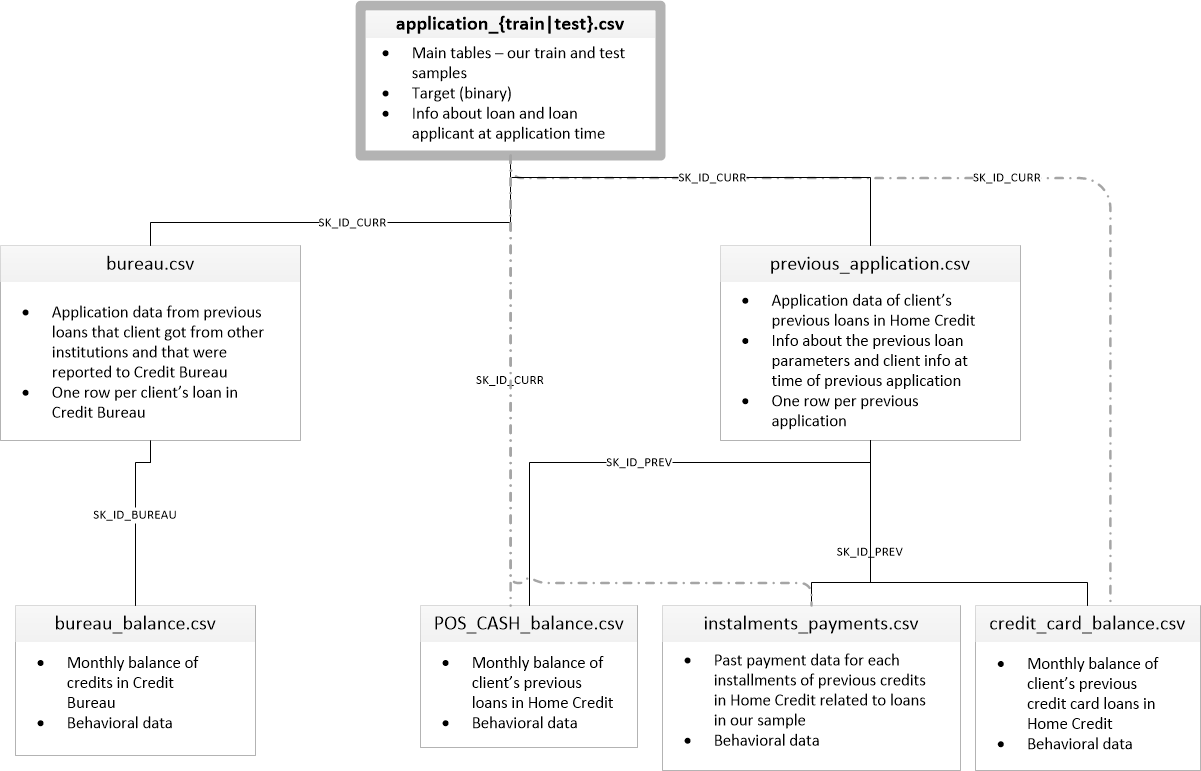
\includegraphics[width=\textwidth]{./home_credit.png}
        \end{column}
    \end{columns}
\end{frame}

\section{Analyse et traitement des données}
\subsection{Exploration du jeu de données}
\begin{frame}{\insertsection}{\insertsubsection}
    \begin{columns}
        \begin{column}{.4\textwidth}
            \begin{itemize}
                \item Certaines colonnes comportent un grand nombre de données manquantes
                      \begin{itemize}
                          \item Nous utiliserons des modèles résistants à ces données manquantes comme XGBoost et LightGBM
                      \end{itemize}
                \item[]
                \item Encodage des variables catégorielles
                      \begin{itemize}
                          \item par LabelEncoder pour les variables ayant 2 catégories
                          \item par pandas.get\_dummies() pour les varibles ayant plus de 2 catégories
                      \end{itemize}
            \end{itemize}
        \end{column}
        \begin{column}{.6\textwidth}
            \includegraphics[width=\textwidth]{app_trainNbDataMiss.pdf}
        \end{column}
    \end{columns}
\end{frame}

\begin{frame}{\insertsection}{\insertsubsection}
    \begin{columns}
        \begin{column}{.5\textwidth}
            \includegraphics[width=\textwidth]{HistPayement.pdf}
        \end{column}
        \begin{column}{.5\textwidth}
            \includegraphics[width=\textwidth]{HistDefAge.pdf}
        \end{column}
    \end{columns}
    \begin{itemize}
        \item L'age des clients semble avoir un impact sur le fait que le client fasse défaut ou non
    \end{itemize}
\end{frame}

\begin{frame}{\insertsection}{\insertsubsection}
    \begin{columns}
        \begin{column}{.33\textwidth}
            \includegraphics[width=\textwidth]{HistSource1.pdf}
        \end{column}
        \begin{column}{.33\textwidth}
            \includegraphics[width=\textwidth]{HistSource2.pdf}
        \end{column}
        \begin{column}{.33\textwidth}
            \includegraphics[width=\textwidth]{HistSource3.pdf}
        \end{column}
    \end{columns}
    \begin{itemize}
        \item Les données EXT\_SOURCE semblent aussi avoir une certaines corrélation avec le fait que le client fasse défaut
    \end{itemize}
\end{frame}

\begin{frame}{\insertsection}{\insertsubsection}
    \begin{columns}
        \begin{column}{.5\textwidth}
            \begin{itemize}
                \item Comme on a pu le voir les données sont déséqulibrées du fait que les clients faisant défauts sont peu nombreux par rapport à ceux ne faisant pas défaut
                \item Classer tous les clients comme ne faisant pas défaut permettrait d'avoir un score honnorable avec seulement 8\% d'erreurs
                \item Nous avons donc utilisé la librairie imblearn qui permet de rééchantillonner notre jeu de données
            \end{itemize}
        \end{column}
        \begin{column}{.5\textwidth}
            \includegraphics[width=\textwidth]{DéséquilibreCible.pdf}
        \end{column}
    \end{columns}
\end{frame}

\subsection{Rééchantillonnage du jeux de données}
\begin{frame}{\insertsection}{\insertsubsection}
    \begin{columns}
        \begin{column}{.5\textwidth}
            \begin{itemize}
                \item Pour essayer les différentes méthodes de rééchantillonnage nous avons réaliser une régression logistique sur les données rééchantiollonnées avec les différents outils
                      \begin{itemize}
                          \item RandomUnderSampler et TomekLinks : méthodes de sous-échantillonnages
                                \begin{itemize}
                                    \item on conserve le même nombre de clients ne faisant pas défaut que de client faisant défaut
                                    \item RandomUnderSampler choisi ces dernier au hasard
                                    \item TomekLinks conserve un certains nombre de clients par groupe de clients similaire (repose sur les KNN)
                                \end{itemize}
                          \item RandomOverSampler et SMOTE : méthodes de sur-échantillonnages
                                \begin{itemize}
                                    \item on multiplie le nombre de clients faisant défaut
                                    \item RandomOverSampler dédouble des clients faisant défaut au hasard
                                    \item SMOTE créé de nouveaux clients à partir de groupe de clients similaires
                                \end{itemize}
                          \item SMOTEENN et SMOTETomek sont des méthodes combinant le sur- et le sous-échantillonnage
                      \end{itemize}
                \item Les scores AUC semblent plutôt bon (\num{>0.7})
            \end{itemize}
        \end{column}
        \begin{column}{.5\textwidth}
            \includegraphics[width=\textwidth]{CurvesROClogreg.pdf}
        \end{column}
    \end{columns}
\end{frame}

\begin{frame}{\insertsection}{\insertsubsection}
    \vspace{2pt}
    \begin{columns}
        \begin{column}{.3\textwidth}
            \includegraphics[width=\textwidth]{CMRandomUnderSampler.pdf}
            \includegraphics[width=\textwidth]{CMSMOTE.pdf}
        \end{column}
        \begin{column}{.3\textwidth}
            \includegraphics[width=\textwidth]{CMRandomOverSampler.pdf}
            \includegraphics[width=\textwidth]{CMSMOTETomek.pdf}
        \end{column}
        \begin{column}{.3\textwidth}
            \includegraphics[width=\textwidth]{CMTomekLinks.pdf}
            \includegraphics[width=\textwidth]{CMSMOTEENN.pdf}
        \end{column}
    \end{columns}
    \small
    \begin{itemize}
        \item Les 2 cas de droites ne sont pas intéressant car le premier classe tout les clients comme ne faisant pas défaut et le second classe 50/50
    \end{itemize}
\end{frame}

\subsection{Création de variables polynomiales}
\begin{frame}{\insertsection}{\insertsubsection}
    \vspace{2pt}
    \begin{columns}
        \begin{column}{.5\textwidth}
            \begin{itemize}
                \item Afin d'améliorer les scores des modèles nous avons essayé de créer des variables polynomiales à partir des colonnes les plus corrélées avec la cible
                \item[]
                \item L'amélioration n'est pas pertinente nous n'avons donc pas conservé ces variables pour notre modèle final
            \end{itemize}
        \end{column}
        \begin{column}{.5\textwidth}
            \includegraphics[width=\textwidth]{ScoresGridFull.pdf}
        \end{column}
    \end{columns}
\end{frame}

\section{Optimisation du modèle}
\subsection{Courbe ROC}
\begin{frame}{\insertsection}{\insertsubsection}
    \begin{columns}
        \begin{column}{.5\textwidth}
            \begin{itemize}
                \item La courbe ROC représente les vrais positifs en fonction des faux positifs
                \item Plus la courbe est proche du coin supérieur gauche meilleur est le modèle
                \item L'aire sous la courbe (AUC) est nous donne une valeur numérique pour comparer ces modèles
            \end{itemize}
        \end{column}
        \begin{column}{.5\textwidth}
            \includegraphics[width=\textwidth]{CurvesROCGridBest_base.pdf}
        \end{column}
    \end{columns}
\end{frame}

\subsection{Différentes métriques utilisées}
\begin{frame}{\insertsection}{\insertsubsection}
    \begin{columns}
        \begin{column}{.5\textwidth}
            \begin{itemize}
                \item Accuracy : précision de la classification (somme des éléments bien classé sur le nombre total d'éléments)
                \item AUC : Area Under the Curve, aire sous la courbe ROC
                \item Precision : part de vrai positifs dans les prédictions positives
                \item Recall : part de vrai positifs dans les éléments vraiments positifs
                \item F1 : moyenne harmonique de la précision et du rappel
                \item F2 : idem F1 avec un facteur β=2, permettant de mettre plus de poid sur le rappel
            \end{itemize}
        \end{column}
        \begin{column}{.5\textwidth}
            \includegraphics[width=\textwidth]{ScoresGrid_base.pdf}
        \end{column}
    \end{columns}
\end{frame}

\subsection{Métrique métier}
\begin{frame}{\insertsection}{\insertsubsection}
    \begin{columns}
        \begin{column}{.7\textwidth}
            \begin{itemize}
                \item But
                      \begin{itemize}
                          \item Diminuer le nombre de faux négatifs (prédit 0, réel 1) afin d'éviter de manquer des clients qui pourraient potentiellement faire défaut
                          \item[$\longrightarrow$] Améliorer le recall
                      \end{itemize}
            \end{itemize}
        \end{column}
        \begin{column}{.3\textwidth}
            \begin{tikzpicture}
                \node[anchor=south west,inner sep=0] (image) at (0,0) { {\makegapedcells
                            \begin{tabular}{cc|cc}
                                \multicolumn{2}{c}{}
                                 & \multicolumn{2}{c}{Prédit}           \\
                                 &                            & 0  & 1  \\
                                \cline{2-4}
                                \multirow{2}{*}{\rotatebox[origin=c]{90}{Réel}}
                                 & 0                          & TN & FP \\
                                 & 1                          & FN & TP \\
                                \cline{2-4}
                            \end{tabular}}};
                \begin{scope}[x={(image.south east)},y={(image.north west)}]
                    \draw[red, ultra thick] (0.7,0.1) circle [x radius=.9cm, y radius=.3cm];
                    \node[rectangle,below] at (0.7,-0.05) (R) {Recall};
                    \draw[green, ultra thick] (0.87,0.25) circle [x radius=.3cm, y radius=.7cm];
                    \node[rectangle,right] at (1,0.25) (P) {Precision};
                    %\draw[help lines,xstep=.1,ystep=.1] (0,0) grid (1,1);
                    %\foreach \x in {0,1,...,9} { \node [anchor=north] at (\x/10,0) {0.\x}; }
                    %\foreach \y in {0,1,...,9} { \node [anchor=east] at (0,\y/10) {0.\y}; }

                \end{scope}
            \end{tikzpicture}
        \end{column}
    \end{columns}
    \begin{columns}
        \begin{column}{.61\textwidth}
            \begin{itemize}
                \item Outil
                      \begin{itemize}
                          \item Utilisation du $F_β$-score qui permet d'ajouter du poid respectivement au recall lorsque le facteur β est \num{>1} ou à la precision lorsque le facteur β est \num{<1}
                          \item Utilisation de β=2
                      \end{itemize}
            \end{itemize}
        \end{column}
        \begin{column}{.39\textwidth}
            \includegraphics[width=\textwidth]{ScoresGridF2_base.pdf}
        \end{column}
    \end{columns}
\end{frame}

\section{Déploiement sur le cloud}
\subsection{API}
\begin{frame}[fragile]{\insertsection}{\insertsubsection}
    \begin{itemize}
        \item Utilisation de Flask
        \item Entrainement du modèle et prédictions
        \item Une URL pour chaque type de données avec une ou plusieurs clé permettant des requêtes sur des clients ou des valeurs particulières
        \item Exemple pour les données des clients pour lesquelles on renseigne l'id du client : \url{http://localhost:5000/ID_clients/infos_client?id=<identifiant>}
        \item[]
    \end{itemize}
    \begin{minted}{python}
@app.route("/ID_clients/infos_client/", methods=["GET"])
def show_data():
    ID_client = request.args.get("id", default=100001, type=int)
    data_client = app_test[app_test.SK_ID_CURR == int(ID_client)].set_index('SK_ID_CURR')
    data_reponse = json.loads(data_client.to_json(orient='index'))
    return jsonify(data_reponse)    
    \end{minted}
\end{frame}

\subsection{Dashboard}
\begin{frame}[fragile]{\insertsection}{\insertsubsection}
    \begin{itemize}
        \item Utilisation de Dashboard
        \item Requêtes à l'API afin d'optenir les données au format JSON
        \item Exemple pour une requête consernant les données d'un client :
        \item[]
    \end{itemize}
    \begin{minted}{python}
URL_API = 'http://localhost:5000/'

@app.callback(Output('infos_client', 'data'), Input('ID_choosed', 'value'))
def get_client_infos(idclient):
    url = URL_API + 'ID_clients/infos_client/?id=' + str(idclient)
    data = requests.get(url).json()
    return data 
            \end{minted}
\end{frame}

\subsection{Déploiement}
\begin{frame}{\insertsection}{\insertsubsection}
    \begin{columns}
        \begin{column}{.4\textwidth}
            \begin{itemize}
                \item Déploiement sur Heroku
                \begin{itemize}
                    \item \texttt{heroku git:remote -a bank-scoring-dash}
                    \item \texttt{git add .}
                    \item \texttt{git commit -am 'launch in the cloud'}
                    \item \texttt{git push heroku master}
                \end{itemize}
            \end{itemize}
        \end{column}
        \begin{column}{.6\textwidth}
            \includegraphics[width=\textwidth]{DashSim.png}
        \end{column}
    \end{columns}
\end{frame}
\end{document}